\section{Modèle discret et implémentation numérique}

On veut minimiser en $\Omega \subset \{1,...,N\}^2$ et en $w \in \mathbb{R}^{N^2}$ la fonctionnelle : 

\[ P(\Omega) + \lambda \sum \limits_{\underset{((m,n), (m, n+1)) \notin \partial \Omega}{\underset{((m,n),(m+1, n)) \notin \partial \Omega}{m,n = 1}}}^{N} |\Delta w_{m,n}|^2 + \mu ||w - u ||_2^2 \]

où $\lambda \geq 0$, $\mu \geq 0$ sont des paramètres et $u \in \mathbb{R}^{N^2}$ est l'image à segmenter. Pour cela, on va utiliser un algorithme de descente sur $\Omega$ et $w$.

\bigskip

Le premier terme de la somme est très proche d'un terme $H^1$, sauf que l'on retire de la somme les points dont le calcul du gradient fait intervenir un voisin de l'autre côté de la frontière de $\Omega$. Ainsi, les points qui ont un très fort gradient tendent à appartenir à la frontière. Le dernier terme constitue l'attache au données. 

\subsection{Notion de périmètre}

On veut minimiser le terme correspondant au périmètre de $\Omega$. Pour définir ce périmètre, on considère un système de voisinage $\sigma(m,n)$ de chaque pixel $(m,n) \in \{1,...,N\}^2$. Les voisinages les plus utilisés sont la 4-connexité définie comme ci dessous :

\[ \sigma (m,n) = \{ (m',n') \in  \{1,...,N\}^2, |m - m' | + |n - n'| = 1 \}\]
Ou la 8-connexité définie comme ci dessous : 
\[ \sigma (m,n) = \{ (m',n') \in  \{1,...,N\}^2, max(|m - m' | , |n - n'| ) = 1 \}\]

\begin{figure}[H]
\centering
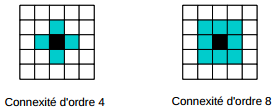
\includegraphics[scale=1]{images/Connexite.png}
\caption{4-connexité et 8-connexité \newline  https://ensiwiki.ensimag.fr/index.php?title=Fichier:Connexite.png}
\end{figure}

On définit alors la frontière de $\Omega \subset \{ 1,...,N\}^2$ comme l'ensemble : 
\[ \partial \Omega = \{ ((m,n),(m',n')) \in (\{ 1,...,N\}^2)^2, (m',n') \in \sigma (m,n) \; et \; (m,n)\in \Omega \; et \; (m',n') \notin \Omega \}\] 

Le périmètre de $\Omega$ est alors définie par : 

\[ P(\Omega) = \sum \limits_{((m,n),(m',n')) \in \partial \Omega} dl((m,n),(m',n')),\] 

Où $ dl((m,n),(m',n')) > 0$ sont des éléments de longueur. Plus la frontière de $\Omega$ contient d'éléments, plus la longueur du contour sera grande. On suppose également pour simplifier que pour tout $((m,n), (m',n')) \in (\{ 1,...,N\}^2)^2$ 

\[ dl((m,n),(m',n')) = dl((m',n'),(m,n))\].

On suppose aussi que 
\[ \text{si} \; (m',n') \notin \sigma (m,n) \; \; \; \text{alors} \; \; dl((m,n),(m',n')) = 0\]

Pour optimiser $\Omega$, on va procéder par des ensemble de niveau.
 
\subsubsection{Représentation de \texorpdfstring{$\Omega$}{Lg}}

Les méthodes basées sur les ensembles de niveaux représentent l'ensemble $\Omega \subset \{1,...N\}^2$ comme un ensemble de niveau d'une image $\phi \in \mathcal{R}^{N^2}$. On pose donc 

\[ \Omega = \{ (m,n) \in \{1,...,N \}^2, \phi_{m,n} \geq 0 \} \].

\subsubsection{Evolution de \texorpdfstring{$\Omega$}{Lg}}

Ainsi, faire évoluer $\Omega$ revient à faire évoluer l'image $\phi$ pour minimiser une énergie analogue mais portant sur $\phi$. On applique un algorithme de gradient à la fonctionelle. On peut donc construire une énergie en $\phi$  pour le terme correspondant au  périmètre tel que : 

\[ E ((\phi_{m,n})_{1 \leq m,n \leq N}) = \sum \limits_{m,n = 0}^N  \sum \limits_{m',n' = 0}^N  dl((m,n),(m',n')) H_{\epsilon} (\phi_{m,n}) ( 1 - H_{\epsilon}(\phi_{m',n'})) \] 
Avec 
\[ H_{\epsilon} (t) = \left\{ \begin{matrix}
1 & \text{si} \; t \geq \epsilon \\
\frac{1}{2} (1 + \frac{t}{\epsilon} + \frac{1}{\pi}sin(\frac{\pi t}{\epsilon})) & \text{si} -\epsilon \leq t \leq \epsilon \\
0 & \text{si} t \leq - \epsilon 
\end{matrix} \right. \] 
Ainsi que son gradient en $\phi = (\phi_{m,n})_{1 \leq m,n \leq N}$ : 

\[ \nabla E (\phi) = ( \sum \limits_{m',n' = 0}^N dl((m,n),(m',n')) H_{\epsilon}' (\phi_{m,n}) ( 1 - 2H_{\epsilon}(\phi_{m',n'}))  ) _{1 \leq m,n \leq N} \] 

Avec 
\[ H_{\epsilon}' (t) = \left\{ \begin{matrix}
0 & \text{si} \; t \geq \epsilon \\
\frac{1}{2 \epsilon} + \frac{1}{2 \epsilon} cos(\frac{\pi t}{\epsilon}) & \text{si} -\epsilon \leq t \leq \epsilon \\
0 & \text{si} t \leq - \epsilon 
\end{matrix} \right. \] 


Ainsi, on combine alors une étape de minimisation d'une énergie sur w, puis d'une étape d'optimisation de la forme $\Omega$, en utilisant un algorithme de descente de gradient. 

\subsection{Convergence de l'algorithme}

\subsubsection{Optimisation de \texorpdfstring{$P(\Omega)$}{Lg}}

L'énergie minimisée ici n'est pas forcément convexe, mais on espère trouver un minimum local. Il est nécessaire de partir d'une bonne initialisation de $\Omega$ pour que le problème d'optimisation ai au moins une solution. 
+ Theoreme 2 page 18 du poly ? pour la convergence 

\subsubsection{Optimisation de la somme}
...
\subsection{Implémentation numérique et résultats}

Présenter les différentes fonctions, leurs interets, algorithme de descente pas constant, résultat, graphique de l'énergie minimisée...